\chapter{Sprint 1}
The first sprint is concerned with getting the semester project started, including both the \gls{astep} project as a whole and the \gls{rs} project.
Thus, the first sprint will be spent on organizing the collaboration with the other project groups and setting the direction for the project.
This means that the contributing parts of sprint 1 will be the initial analysis, requirement specification and overall design, with the documentation in this chapter in the same order.

\section{Analysis}
Ridesharing is an activity which has had phases of popularity in recent history according to \citet{doi:10.1080/01441647.2011.621557}.
They describe the current phase as the technology-enabled ridematching phase which started in 2004.
In this phase, the intergration of the internet, mobile phones, and social media has into ridesharing services, reduces the barrier to entry for new potential passengers and drivers.
\citet{doi:10.1080/01441647.2011.621557} also list incentives for ridesharing in the current phase, which are as follows 

\begin{itemize}
  \item ``Focus on reducing climate change, growing dependence on foreign oil, and traffic congestion
  \item Partnerships between ridematching software companies and regions and large employers
  \item Financial incentives for green trips through sponsors
  \item Social networking platforms that target youth
  \item Real-time ridesharing services'' \citep{doi:10.1080/01441647.2011.621557}.
\end{itemize}

This presents a broad overview of why ridesharing became popular again after 2004.
Because technologies play a vital role in the current phase a selection of popular commercial services will be examined a long with some scientific papers to get a comprehension of the state of the art in the field.
%The following section documents the analysis of both academic papers, as well as corporate and community products, to get a comprehension of the state of the art in the ridesharing field.
The main focus will be on real-time or dynamic ridesharing which \citet{amey2011real} defined as ``rideshare service relying heavily on mobile phone technologies''.

\subsection{Scientific Papers}
The problem of automating ridesharing through modern technology has already been studied by multiple scientists \todo{what?} with different approaches.
The following sections account for some of which we found the most interesting and relevant to the problem statement. 

\citet{doi:10.1080/01441647.2011.621557, amey2011real} sees technology as one of the most important factors in the present and future of dynamic ridesharing.

\citet{ShuoMa2013} developed an algorthm for taxi services which improved throghput of passengers by 25\% and reduced the distance a single taxi had to drive by 13\% when there where there were six requests for rides per taxi. %  picking up many passengers throughout a ride is developed and presented, seeking to increase the passenger throughput as well as lowering the distance traveled per passenger served.
Especially interesting in their paper is an approach which suggests a grid representation of a road network, this is to avoid shortest path calculations between points on a map, and instead approximate distance represented by cells in the grid.
The paper also uses	 the user's smartphone to collect location data and act as a user interface.

\citet{ghoseiri2011real} researched what might matter when matching driver and passengers.
They focused on preferences which influence whether you want to drive with a person, this can be everything from gender to pet friendliness.
They developed functions which assesses whether a passenger and driver match, based on location, preferences, passenger and/or driver detour as the most important factors \cite{ghoseiri2011real}.
This algorithm might be useful in this project solution.

Actual choices and influences regarding algorithm design for ridematching will be addressed in the design phase. 

\subsection{Commercial Solutions}
Corporate and community solutions are quite different from the academic field.
The main focus seems to be centered around taxi alternatives.
The two biggest international services in this field as of 2016 is Uber and Lyft\todo{source}.
There are also several services with some or all of their focus in Denmark, most notable is services like Haxi and Drivr\todo{source}.
These services work in a similar way: 

\begin{enumerate}
	\item A customer request a ride through an smartphone app or a web interface
	\item The backend of the service sends the request to one or more appropriate drivers
\end{enumerate}

Since the mentioned services are commercial and closed-source, actual information about the services design or architecture is not available.
Drivr has two interesting feature in comparison to their opponents, that is a web system for fleet management and business which provides administration and expense control of employee taxi travels.

Besides these taxi like services, there also exist services which focus on traditional ridesharing between private people where money is not earned.
Again, here exist both local and international services. 
These services give the opportunity to either offer a lift, request a ride and the possibility to connect drivers and passengers.
These services are usually free, but some of them charge a small fee when connecting people.
Some of the more notable are GoMore and iRideshare.\todo{source}

The smartphones have automatized much of the labor concerning organizing ridesharing and act as a central component in all the analyzed systems\todo{what?}.
However, we still see an opportunity to use the smartphone even further in a service that arranges rides between users, thus decreasing the required labor.
\section{Requirement Specification}\label{sec:req}
% Metatext
The requirements are divided into two main categories, functional and nonfunctional requirements, and are furthermore sorted in the MoSCoW \cite{moscow} structure.
The structure assists in solving the core purpose of the system first, as these are the highest prioritized requirements, and later adding additional functionality.


% Requirements
\subsection{Functional requirements}
The functional requirements are directly related to the tasks and operations of the developed application.

\textbf{Must-have requirements}\\
The 'Must have' requirements must be fulfilled for the solution to be acceptable.

\textit{Graphical user interface}\\
The application must have a graphical user interface (GUI) as users must be able to use the application themselves, and to structurally and aesthetically display user matches. 
The GUI must be intuitive as users may have different levels of experience with using mobile applications.

\textit{User accounts, including login and registration.}\\
Unique user accounts are required as it serves as an identifier for each user in the system. 
With user accounts, store personal information, and compare user based on the data. 
It will also provide functionality for displaying user to other users.

\textit{Communication with the \gls{astep} system.}\\
As the project is a part of the bigger system \gls{astep}, there must be a relation to the developed platform. 
The communication would be storing data in the \gls{astep} database and using user management also implemented on the platform.

\textit{User location tracking and storage.}\\
The application must track users as they move, to be able to determine the users travel routes.
The application should store the commuted routes and the data should be stored in the \gls{astep} database.

\textit{Automatically determine regular routes.}\\
The solution must automatically determine if a route is regular. 
Regular routes should be used for route comparison and match generating. 

\textit{Automatic user ridesharing suggestions.}\\
Automatic matching with other users routes must be provided to the the individual app users, and the matches must be computed.
When two regular routes are found similar, the users must receive an indication of the match in the app.
If the match computation shows to be a excessive process it is deemed to be done in the \gls{astep} core.


\textbf{Should-have requirements}\\
The requirements in this subsection are important, but are not regarded as critical for the functionality of the solution.

\textit{Give the user option to specify whether they have a car or not.}\\
Because some users might not have a car, they should be considered differently than the ones with, as the users without vehicle cannot give a ride to a potential match.

\textit{Enable users to blacklist other users.}\\
Users should be able to filter other users from the matches to prevent further possible bad experiences with either a driver or passenger.

\textit{Suggest rides with users who only drives a subset of the way from A to B.}\\
Giving users the option to match with people who do not have the same source and destination, will increase the number of suggested matches, as a user can join a part of the matches' route.


\textbf{Could-have requirements}\\
The 'Could have' requirements are the lowest realistically fulfillable requirements, and are implemented if the higher priority requirements are fulfilled.

\textit{Ride reservation or request from, to, time.}\\
This requirement enables the user to reserve rides with other users. 

\textbf{Would-have requirements}\\
The following requirements are only considered when all other requirements are satisfied but initially regarded as tasks to be solved in future projects.

\textit{Inform users of their environmental and economic savings due to their use of the solution.}\\
Provide users with detailed information on how much fuel the user has saved, how much money saved based on fuel prices, and how much CO2 that is not released into the environment. 

\subsection{Non-functional requirements}
The nonfunctional requirements for the solution are stated here.

\textbf{Must-have requirements}\\
These are the requirements the solution must fulfill to be acceptable.

\textit{Development cooperation with the other \gls{astep} project groups.}\\
The development must be done in cooperation with the other \gls{astep} groups.

\textit{User privacy}\\
The app must respect user privacy, especially in regards to a user location data and personal user data.
The solution should consider securing elements such as database storage, user management, and developers.

\textbf{Should-have requirements}\\
These requirements are important, but are not regarded as highly critical.

\textit{Aesthetics matching other \gls{astep} project applications}\\
The app should share design and guidelines as the other apps developed for \gls{astep}.

As the requirements for the solution now are documented the first design phase can be initiated. 
\section{Design}\label{sprint1design}
% Metatext
This section contains the overall app design, which is based on requirements with inspiration taken from the different commercial products and the papers read in the analysis.
The section will outline the main features of the design concerning system's structure, components, and user interface.

\subsection{System design}
To exploit the availability of sensors on the mobile phone and computational power of the server, the system is developed in two parts: the phone application and an extension of the route system in the \gls{astep} system which handles the analysis and comparison of routes.
The two parts will have their own delegated responsibilities, and will perform the necessary tasks, enabling the system to deliver the service.

% The app
\textbf{The \gls{rs} App}\\
The application, hereafter referenced as the app, is the program executed on a mobile device.
Its responsibilities include the gathering of location data and providing the user interface. 

% device limitations -> app abilities
The task of comparing routes is assumed to require much processing power, and also be able to access location data to get the aforementioned routes.
Performing the route comparisons in the app would require that each user have a copy of every other user's routes.
This is a serious privacy concern as this can enable other applications to leach on to the \gls{astep} system a gather data about when people are home and where they live, and is an aspect we would like to avoid.
As mentioned before, calculating the best route matches would most likely require a lot of processing power, which would drain the battery and produce heat.

Assuming that a central server can handle the analysis of the routes, the application is only required to supply the server with location data.
This is a much better solution as the impact on the battery is reduced, and private information can be contained within the \gls{astep} system.

A service running in the background of the app can handle the location data sampling and transfer to a server.
This service would be kept alive when the application is closed as its own thread, thus being able to record routes even when the app is not in focus on the device.
Because the main objective of the background service is to observe the current activity and transfer the route to \gls{astep}, we call it Observer.
The structure of the class can be seen in Figure \ref{fig:classDiagramSprint1Observer}.
The Observer's main goal is to observe what activity the user is currently performing and receive and push locations accordingly.
There are already implementations for this kind of service in Google Play Services for Android applications and these will be utilized.

\begin{figure}[h]
	\centering
	\begin{tikzpicture}[auto]
	\node[class](Observer){Observer
		\nodepart[align=left, text width=4.1cm]{two}
		-currentActivity : Integer
		\nodepart[align=left, text width=4.1cm]{three}
		+observerActivity() : Integer};
	\node[class, below=of Observer](RouteBuilder){RouteBuilder
		\nodepart[align=left, text width=4.9cm]{two}
		-locations : Location[]\\
		-user : UserInfo
		\nodepart[align=left, text width=4.9cm]{three}
		+RouteBuilder(user : UserInfo)\\
		+addLocation(location : Location)\\
		+buildRoute() : Route};
	\draw[aggregation] (Observer) -- (RouteBuilder);
\end{tikzpicture}
	\caption{The small process which should run at all time to build the routes.}
	\label{fig:classDiagramSprint1Observer}
\end{figure}

The API does also have features for detecting which activity is currently being performed.
This can be used to stop and start the gathering of location data, depending on the given activity.

% The aSTEP core
\textbf{The \gls{astep} Component}\\
On the \gls{astep} server, the route is stored in a database and accessed by the RouteStabilityAnalyser.
This analyzer takes the route and compares it to other routes by the same user, to determine whether this route is a regular occurrence, and hence a stable route.

If the RouteStabilityAnalyser determines that the route is stable, the route should be marked with a tag indicating that the route is stable in the database together with values that indicate when this route is expected to occur next.
The server then uses the RouteSimilarityAnalyser to find matches for the new StableRoute.
The matches are stored and new matches are transmitted to the appropriate devices when possible to inform the users of new matches.

%\begin{figure}[h]
%	\centering
%	\begin{tikzpicture}[auto]
	\node[class](LoginActivity){LoginActivity
		\nodepart[align=left, text width=2.7cm]{two}
			-username : String\\
			-password : String
		\nodepart[align=left, text width=2.7cm]{three}
			+submit()};
	\node[class, below left=1 and -1 of LoginActivity](RegisterActivity){RegisterActivity
		\nodepart[align=left, text width=2.7cm]{two}
			-username : String\\
			-password : String
		\nodepart[align=left, text width=2.7cm]{three}
			+submit()};
	\node[class, below right=1 and -1 of LoginActivity](MainActivity){MainActivity
		\nodepart[align=left, text width=4cm]{two}
			-currentUser : UserInfo
		\nodepart[align=left, text width=4cm]{three}
			+MainActivity(user : UserInfo)\\
			+fetchSuggestedRoutes()};
	\node[interface, right=of MainActivity](ISuggestedRoute){
		\nodepart[align=center, text width=2.8cm]{one}
			<<interface>>\\
			ISuggestedRoute
		\nodepart[align=left, text width=2.8cm]{two}
			-getRoute() : Route};
	\node[class, below=of ISuggestedRoute](SuggestedRoute){SuggestedRoute
		\nodepart[align=left, text width=2.8cm]{two}
			-getRoute() : Route};
		
	\draw[association, dashed] (LoginActivity) -| (MainActivity);
	\draw[association, dashed] (LoginActivity) -| (RegisterActivity);
	\draw[association, dashed] (RegisterActivity) -- (MainActivity);
	\draw[generalization, dashed] (SuggestedRoute) -- node[label] {<<realize>>} (ISuggestedRoute);
	\draw[aggregation](MainActivity)--(ISuggestedRoute);
	
	\node[draw, fit=(MainActivity) (LoginActivity) (RegisterActivity)](PackageBody){};
	\node[draw, above right] at(PackageBody.north west){activities};
\end{tikzpicture}
%	\caption{The class structure of the application.}
%	\label{fig:classDiagramSprint1Application}
%\end{figure}

This is the start of a project that will be further developed upon and expanded in the future, emphasizing the importance of reuse in the server, to reduce the number of specialized server resources.
By isolating parts that are specific to the rideshare app on the server, most of this system would be reusable.
An example of how this is achieved through object-oriented design, is the RouteAnalyser seen in Figure \ref{fig:classDiagramSprint1Server}.
The RouteAnalyzer filter routes according to its concrete implementation.
After the filtering, the RouteAnalyser compare the routes.
This enables other projects to develop their own filters and comparison functions for later projects.

\begin{figure}[h!]
	\centering
	\begin{tikzpicture}[auto]
	\node[class](Route){Route 
		\nodepart[align=left, text width=6.3cm]{two}
			-id : Integer\\
			-user : UserInfo\\
			-points : Location[]
		\nodepart[align=left, text width=6.3cm]{three}
			+Route(user : UserInfo, points : Location[])\\
			+getUser() : UserInfo\\
			+getPoint(index : Integer) : Location};
	\node[class, below=of Route](StableRoute){StableRoute
		\nodepart[align=left, text width=6.3cm]{two}
			-days : WeekDays\\
			-departureTime : Time\\
			-arrivalTime : Time
		\nodepart[align=left, text width=6.7cm]{three}
			+StableRoute(route : Route, days : WeekDays)\\
			+getArrivalTime() : Time\\
			+getDepartureTime() : Time};
	\node[class, below=of StableRoute](RouteStabilityAnalyser){RouteStabilityAnalyser
		\nodepart[align=left, text width=4.6cm]{two}
			-isStable : Boolean\\
			-currentRoute : Route
		\nodepart[align=left, text width=4.6cm]{three}
			+getStableRoute() : StableRoute\\
			+analyse(route : Route)};
	\node[class, right=of StableRoute](RouteAnalyser){\textit{RouteAnalyser}
		\nodepart[align=left, text width=3.4cm]{two}
			-id : Integer
		\nodepart[align=left, text width=3.4cm]{three}
			+analyse(route : Route)};
	\node[class, right=of RouteStabilityAnalyser](RouteSimilarityAnalyser){RouteSimilarityAnalyser
		\nodepart[align=left, text width=3.4cm]{three}
			+analyse(route : Route)};
	\node[interface, below=5 cm of RouteAnalyser](RouteComparer){
		\nodepart[align=center, text width=4cm]{one}
		<<interface>>\\
		IRouteComparer
		\nodepart[align=left, text width=5.9cm]{two}
			+compare(x : Route, y : Route) : Integer};
	\node[class, below=of RouteComparer](TimeDistanceComparer){TimeDistanceComparer
		\nodepart[align=left, text width=5.9cm]{three}
			+compare(x : Route, y : Route) : Integer};
	
	\draw[aggregation,transform canvas={xshift=1.3cm}] (RouteAnalyser) -- (RouteComparer);
	\draw[association, dashed,transform canvas={xshift=-1.3cm}] (RouteStabilityAnalyser) -- node[label]{<<build>>} (StableRoute);
	
	\draw[generalization] (StableRoute) -- (Route);
	\draw[generalization] (RouteStabilityAnalyser.north) -- ++(0,0.5) -| (RouteAnalyser);
	\draw[generalization] (RouteSimilarityAnalyser.north) -| (RouteAnalyser);
	\draw[generalization, dashed] (TimeDistanceComparer) -- node[label]{<<realize>>} (RouteComparer);
	\draw[association] (RouteAnalyser) |- node[label, at end, xshift=0.3cm]{0..*} (Route.east);
\end{tikzpicture}
	\caption{The structure of the system inside the server.}
	\label{fig:classDiagramSprint1Server}
\end{figure}

Because commuters were our target and commutes are most likely to occur on a weekly basis, a weekly stability was decided upon.
This means that the RouteStabilityAnalyser can be limited to analyze only two months of data, as the route can be stopped driven.

\subsection{User Interface Design}
% General Introduction to UI - what + why
The \gls{ui} provides interaction methods between the user and the app.
As the priority of this project is functionality with regards to data collection and route generation and comparison, the \gls{ui} will not be developed together with users, nor allocated excessive resources. 
The \gls{ui} is developed for practical purposes, such as testing, and to lay the basis for further development, but is still held to a usable standard which will be documented in the following sections. 

\subsubsection{Design language}
% Definition
The design language is the general look and appearance of a system.
This is the foundation for the user impressions and affects the user experience.
The design language is selected in collaboration with another aSTEP project group, SW604F16.

% Goals
The user interface is designed to achieve the following usability characteristics described by \citet{DIS2014}:
\begin{itemize}
	\item Learnability
	\item Utility
	\item Safety
	\item Effectiveness
\end{itemize}

% Material design
The \gls{ui} is designed to comply with the Google's Material design guidelines \cite{materialDesign}, being ``\textit{bold, graphic, intentional}''. 
Some of the Material design properties are stated in the following list, compiled of citations from the design guidelines \cite{materialProperties}:

\begin{enumerate}
	\item Material has varying x \& y dimensions (measured in dp) and a uniform thickness (1dp).
	\item Material casts shadows. Shadows result naturally from the relative elevation (z-position) between material elements.
	\item Content is displayed on material, in any shape and color. Content does not add thickness to material.
	\item Input events cannot pass through material.
	\item Material cannot pass through other material. For example, one sheet of material cannot pass through another sheet of material when changing elevation.
	\item Material grows and shrinks only along its plane.
	\item Material never bends or folds.
	\item Material can be spontaneously generated or destroyed anywhere in the environment.
\end{enumerate} 

% Paragraph regarding selection of material
Adhering the material design guidelines makes the app achieve a similar aesthetic and usage method as other apps in the Android eco-system. 
The design language aims to make the interface clean and simple, regarding colors and input methods.

\subsubsection{User interface}
% Actions in UI and design thereof
This section contains design drafts of the user interface style and functionality.
The design drafts in Figure \ref{fig:GUI-firstrun} reflect the necessary functions and the previously described design language. 

% Login and registering pages design
As the user needs a user profile in the \gls{astep} system to use the app, the users must be able to log in if they have a user profile, and create a new user profile if they are not already registered.

\begin{figure}[h!]
	 \centering
	 \begin{subfigure}[b]{0.3\textwidth}
	 	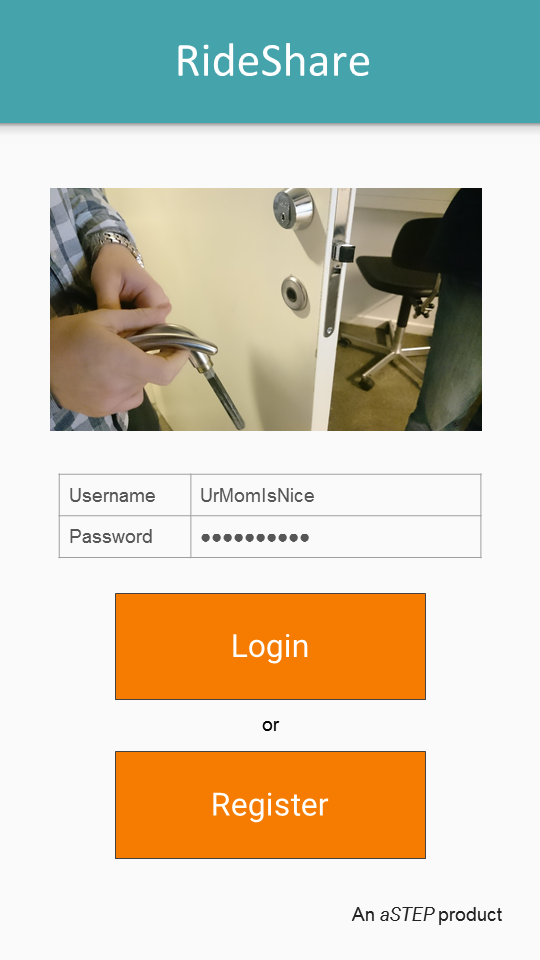
\includegraphics[width=\textwidth]{figures/GUI-front.png}
	 	\caption{Login page}
	 	\label{fig:GUI-front}
	 \end{subfigure}
	 ~ %add desired spacing between images, e. g. ~, \quad, \qquad, \hfill etc. 
	 %(or a blank line to force the subfigure onto a new line)
	 \begin{subfigure}[b]{0.3\textwidth}
	 	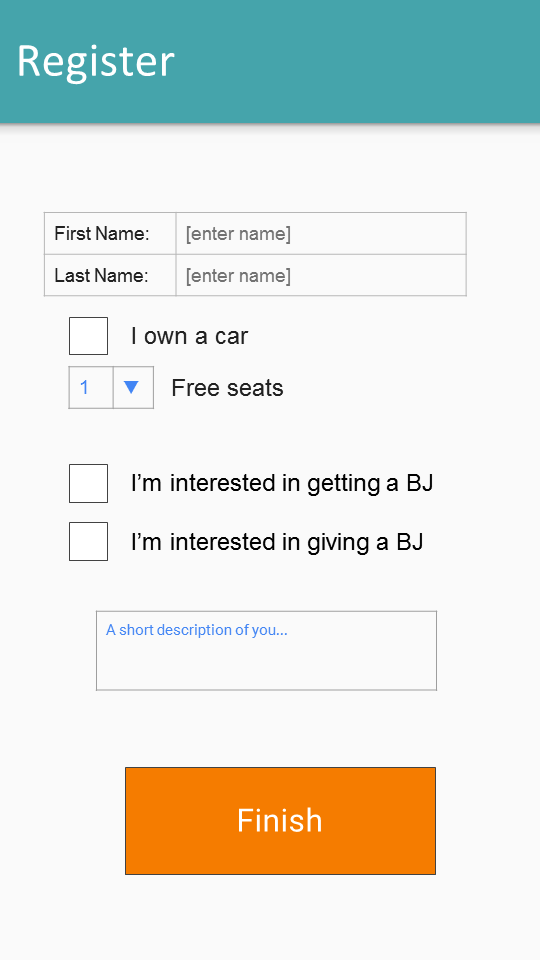
\includegraphics[width=\textwidth]{figures/GUI-register.png}
	 	\caption{Register page}
	 	\label{fig:GUI-register}
	 \end{subfigure}
	 ~ %add desired spacing between images, e. g. ~, \quad, \qquad, \hfill etc. 
	 %(or a blank line to force the subfigure onto a new line)
	 \begin{subfigure}[b]{0.3\textwidth}
		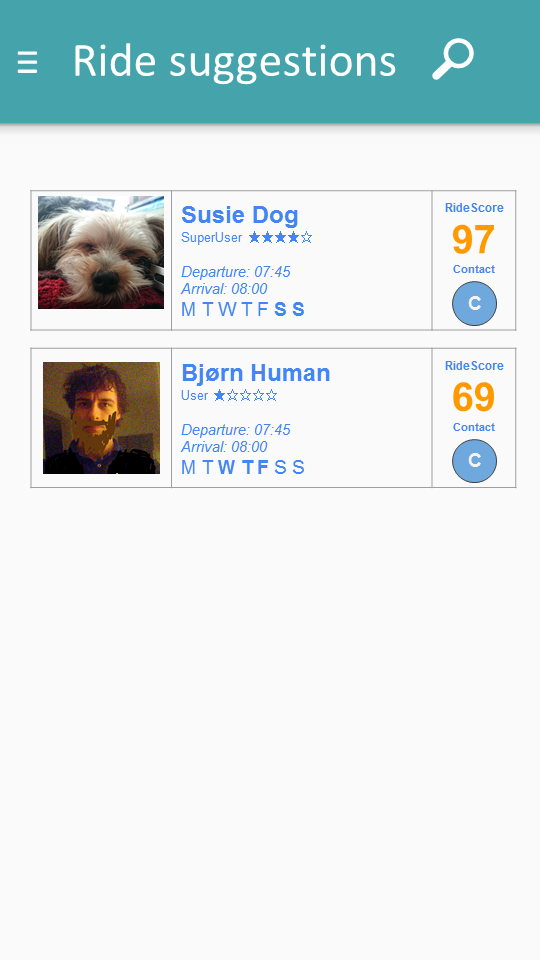
\includegraphics[width=\textwidth]{figures/GUI-main.png}
		\caption{Main page}
		\label{fig:GUI-main}
	\end{subfigure}
	 \caption{Draft of the views in the app.}\label{fig:GUI-firstrun}
\end{figure}

% In-app pages design
Several views are necessary to support the different parts of the app. 
The app needs views for login, registering, and presentation of matches as can be seen in the figures in Figure \ref{fig:GUI-firstrun}.

The application must be able to show matches in a separate view.
In this view, the user will be presented a list of other users which most likely are good matches. 
The users listed should be in a descending order, with the highest rated match at the top.
A short description of the users and match should be displayed, such as the user's full name, phone number, the match score, and what day(s) of the week the user drove the route and is expected to drive again.

This concludes the design of the app.
As earlier mentioned, the \gls{ui} is not the main focus of the project and will therefore not be further developed for other than functional purposes.

%\begin{figure}[h!]
%	\centering
%	\begin{subfigure}[b]{0.3\textwidth}
%		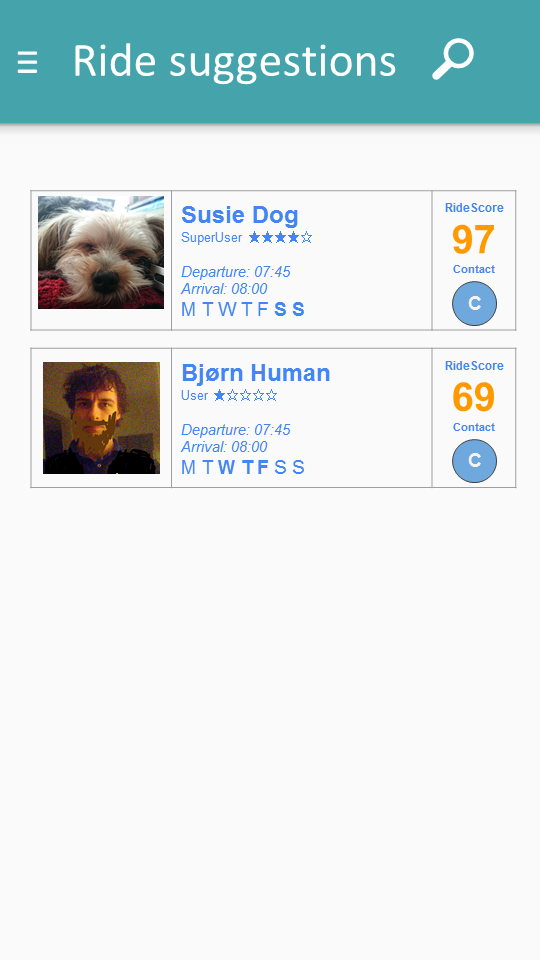
\includegraphics[width=\textwidth]{figures/GUI-main.png}
%		\caption{Main page}
%		\label{fig:GUI-main}
%	\end{subfigure}
%	~ %add desired spacing between images, e. g. ~, \quad, \qquad, \hfill etc. 
%	%(or a blank line to force the subfigure onto a new line)
%	\begin{subfigure}[b]{0.3\textwidth}
%		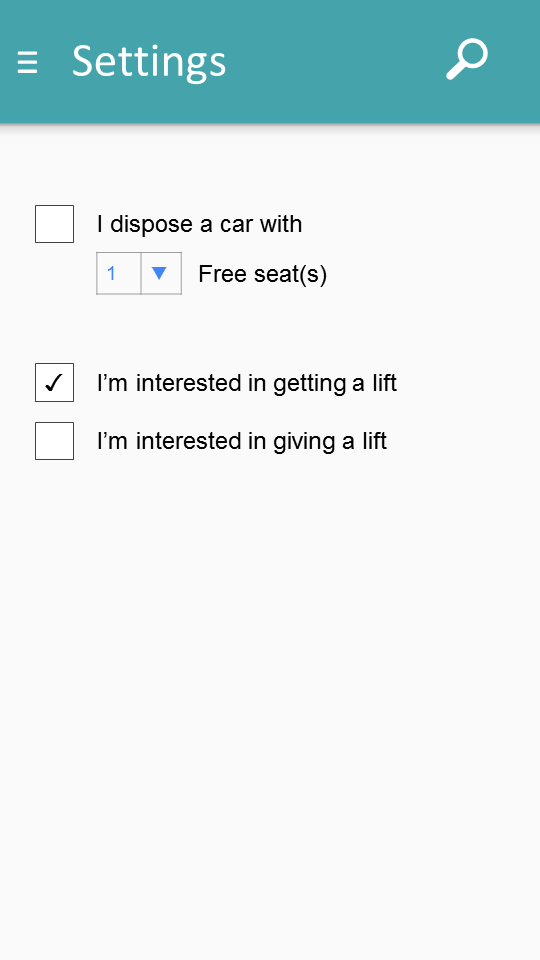
\includegraphics[width=\textwidth]{figures/GUI-settings.png}
%		\caption{Settings page}
%		\label{fig:GUI-settings}
%	\end{subfigure}
%	\caption{Draft of the views in the app.}\label{fig:GUI-in-app}
%\end{figure}
%\section{Implementation}
%\section{Test}